%課題研究レジュメテンプレート ver. 1.0

\documentclass[uplatex]{jsarticle}
\usepackage[top=20mm,bottom=20mm,left=20mm,right=20mm]{geometry}
\usepackage[T1]{fontenc}
\usepackage{txfonts}
\usepackage{wrapfig}
\usepackage[expert,deluxe]{otf}
\usepackage[dvipdfmx,hiresbb]{graphicx}

\makeatletter
  \renewcommand{\section}{%
    \if@slide\clearpage\fi
    \@startsection{section}{1}{\z@}%
    {\Cvs \@plus.5\Cdp \@minus.2\Cdp}% 前アキ
    {.5\Cvs \@plus.3\Cdp}% 後アキ
    %{\normalfont\Large\headfont\raggedright}}
    {\normalfont\raggedright}}

  \renewcommand{\subsection}{\@startsection{subsection}{2}{\z@}%
    {\Cvs \@plus.5\Cdp \@minus.2\Cdp}% 前アキ
    {.5\Cvs \@plus.3\Cdp}% 後アキ
    %{\normalfont\large\headfont}}
    {\normalfont}}

  \renewcommand{\subsubsection}{\@startsection{subsubsection}{3}{\z@}%
    {\Cvs \@plus.5\Cdp \@minus.2\Cdp}%
    {\z@}%
    %{\normalfont\normalsize\headfont}}
    {\normalfont}}
\makeatother
%ここから上を編集する必要はない.



\usepackage{url}
%↑ネットから



\title{\vspace{-14mm}Wikipediaの履歴データ解析}
\author{PMコース 矢吹研究室 1242005 石井康之}
\date{}%日付を入れる必要はない.
\pagestyle{empty}%ページ番号は振らない.
\begin{document}
\maketitle





\section{研究の背景}

Wikipediaはオープンなプロジェクトにおける最も有名な成功事例のひとつである\cite{test1}.使用頻度が高いサイトで,約10年も続いているほどの古参サイトである.また多言語で展開されており,2014年12月1日で288言語も開設され,記事の数なら総合計で3000万件を超えた\cite{test107}.Wikipediaは誰でも自由に編集できる百科事典なので,内容の信頼性を疑問視する声もある.問題のある記述がなされた場合,それは善意のある人に一任される.完全な自由主義なため悪意のある人の編集を防ぎきれないという指摘がある.記事は完成・確定されることはないので,新しい情報にいつでも改変することができる.

Wikipediaについて調査することで,オープンなプロジェクトのマネジメントについての知見が得られることが期待される.誰でも自由に編集できる状況において,どのように品質管理がなされているのか調査する.また多くの執筆者の協力によって成り立っているプロジェクトなので,どのように人的資源が活用されているのか調査する.

Wikipediaのデータは膨大なため,調査のためにはビッグデータを扱う技術が必要である.ビッグデータとは市販されているデータベース管理ツールや従来のデータ処理アプリケーションで処理することが困難なほど巨大で複雑な データ集合の集積物を表しているものだ\cite{test106}.適切なハードウェアと適切な環境を用意しないと,個人で扱うには時間と費用が多くかかってしまう.

そこで本研究では,Wikipediaを調査できるようなビッグデータ処理技術を調査し,そのベンチマークを行う.この調査により,オープンなプロジェクトにおけるマネジメントのあり方について調査するための技術を身につける.





\section{研究の目的}

ビッグデータを解析できる技術を取得することを目指す.Wikipediaの膨大な編集履歴データを扱えるようにするためである.



\section{プロジェクトマネジメントとの関連}

Wikipediaを1つのプロジェクトとみなすと,品質管理マネジメントと人的資源マネジメントの2つを関連付けられる\cite{test8}.

品質管理マネジメントに関連付くと考えられるのは,オープンな共同作業のプロジェクトにおいて,ふさわしくない投稿を繰り返し続ける行為の荒らしや,話し合いをせず他者の編集を繰り返し差し戻しを行う編集合戦があるにもかかわらず,現在では誰もが信頼して使うような百科事典になったためである.

人的資源マネジメントに関連付くと考えられるのは,多くのボランティアの人々の協力により,Wikipediaが多くの情報を持つ百科事典になったためである.






\section{研究の方法}

本研究ではXML dump\cite{test105}とGoogle BigQuery\cite{test104}を利用する.

XML dumpとは,Wikipediaのすべての記事の完全な編集履歴を提供しているものである.これを利用して研究で必要なWikipediaであげられているデータを取得する.

Google BigQueryとは,大量のデータに対して高速にクエリを実行可能なGoogleのサービスで,クラウドにあるビッグデータをSQLを使って解析できる.これを利用してXML dumpに入っている編集履歴からデータ解析を行う.

これらを用いて,以下のように研究を進める.

\begin{enumerate}
\item BigQueryの利用の仕方を調べる\cite{test102}.

\item BigQueryを用いてWikipediaの作業履歴データを取得する.

\item BigQueryを用いてWikipediaの作業履歴データを利用できるようにする.(XML dumpからデータを抽出し,解析できるようにもする)

\item BigQueryの処理技術のテストとして記事ごとの差し戻し履歴の統計を取る.

\item BigQueryを用いて抽出したデータと,差し戻し履歴の統計を参考にしているサイト\cite{test103}を照らし合わせて一致しているか確認する.
\end{enumerate}





%\begin{wraptable}[行数]{r}{幅}%行数はオプションだが,調整しないとうまくいかない.
\begin{wraptable}[12]{r}{10cm}
\vspace*{-\intextsep}
\caption{差し戻し回数の比較 両記事とも回数が多い順に出している}\label{サンプル表}
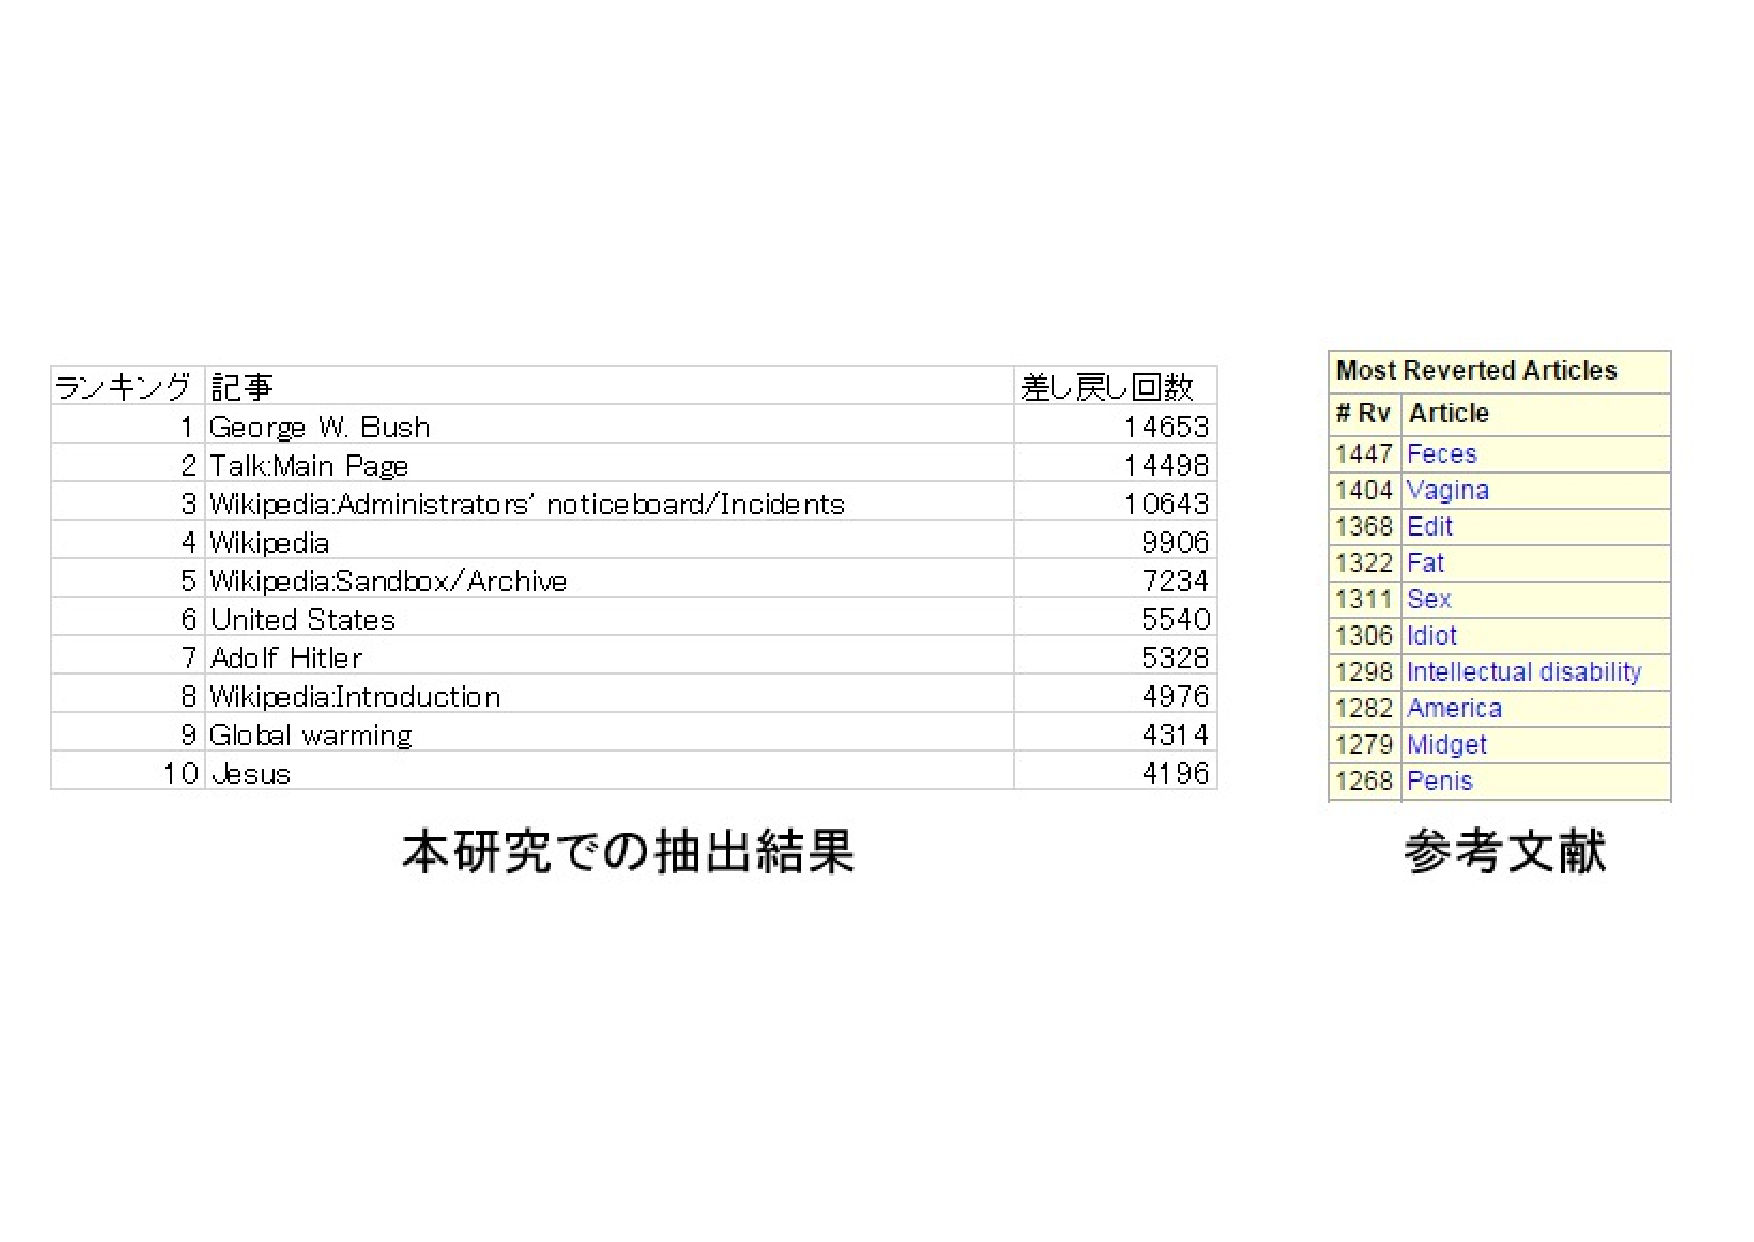
\includegraphics[width=10cm,clip]{revert3.pdf}
\end{wraptable}



\section{現在の進捗状況}

以下のように進んでいる.

\begin{enumerate}
\item BigQueryを用いてWikipediaの履歴データを解析した.
\item BigQueryを用いて履歴データの中から差し戻し履歴の部分を記事ごとに抽出し,ランキングを作成した.
\item 差し戻し履歴の統計が参考にしているサイトと照らし合わせたら一致しなかったので,原因を調査した.
\item 扱っていたデータの範囲はほぼ同じだった.差し戻し履歴の抽出方法が違っていたと考察する.
\end{enumerate}





\section{今後の計画}

以下のように進める予定である.

\begin{enumerate}
\item Wikipediaの全編集履歴データをダウンロードする.
\item 引き続きBigQuery,またはAPIを用いて解析する.
\item Wikipediaの各記事の差し戻し回数の集合知を描き,どのような傾向があるか調査する.
\end{enumerate}



\bibliographystyle{junsrt}
\bibliography{biblio}%「biblio.bib」というファイルが必要.

\end{document}